% Źródła: materialy/2026-10-29/IMG_7038--IMG_7043.jpeg.
\poczatekwykladu{5}

\section{Funkcje niezależnych zmiennych losowych}
\label{sec:funkcje-niezaleznych-zmiennych}

\begin{twierdzenie}
\label{tw:funkcje-niezaleznych-blokow}
Niech $X_1,\ldots,X_{n+m}$ będą niezależnymi zmiennymi losowymi,
gdzie $n,m\geq1$. Wówczas dla dowolnych zbiorów borelowskich
$C\in\B(\R^n)$ i $D\in\B(\R^m)$ zdarzenia
\[
  \{(X_1,\ldots,X_n)\in C\},
  \qquad
  \{(X_{n+1},\ldots,X_{n+m})\in D\}
\]
są niezależne. W szczególności, jeżeli funkcje
\[
  f\colon\R^n\to\R,
  \qquad g\colon\R^m\to\R
\]
są borelowskie, to zmienne losowe
\[
  f(X_1,\ldots,X_n),
  \qquad g(X_{n+1},\ldots,X_{n+m})
\]
są niezależne.
\end{twierdzenie}

\begin{uwaga}[Więcej bloków]
\label{uwaga:wiecej-niezaleznych-blokow}
Ogólniej, niech $X_1,\ldots,X_n$ będą niezależne oraz
\[
  0=n_0<n_1<\cdots<n_k=n.
\]
Jeżeli dla $i=1,\ldots,k$ funkcje
$f_i\colon\R^{n_i-n_{i-1}}\to\R$ są borelowskie, to zmienne
\[
  f_1(X_1,\ldots,X_{n_1}),\quad
  f_2(X_{n_1+1},\ldots,X_{n_2}),\quad\ldots,\quad
  f_k(X_{n_{k-1}+1},\ldots,X_n)
\]
są niezależne.
\end{uwaga}

\begin{przyklad}
Jeżeli $X_1,X_2,X_3$ są niezależne, to
$\sin(X_1+X_2)$ i $e^{X_3}$ są niezależne.
Podobnie z niezależności $X_1,X_2,X_3,X_4$ wynika niezależność
zmiennych $X_1+X_2$ oraz $X_3-X_4$.
\end{przyklad}

\begin{uwaga}
Twierdzenie dotyczy funkcji oddzielnych bloków zmiennych.
Z samej niezależności $X_1$ i $X_2$ nie można wnioskować,
że zmienne $X_1+X_2$ oraz $X_1-X_2$ są niezależne.
\end{uwaga}

\begin{proof}[Szkic dowodu twierdzenia~\ref{tw:funkcje-niezaleznych-blokow}]
Oznaczmy
\[
  X=(X_1,\ldots,X_n),
  \qquad Y=(X_{n+1},\ldots,X_{n+m}).
\]
Chcemy wykazać, że
\begin{equation}
  \PP(X\in C,\,Y\in D)=\PP(X\in C)\PP(Y\in D)
  \label{eq:niezaleznosc-blokow}
\end{equation}
dla wszystkich $C\in\B(\R^n)$ oraz $D\in\B(\R^m)$.

Dla $d\geq1$ rozważmy rodzinę prostokątów
\[
  \mathcal A^d=
  \left\{\prod_{i=1}^d[a_i,b_i):
    a_i,b_i\in\R,\ a_i\leq b_i\right\}.
\]
Jest to $\pi$-układ i $\sigma(\mathcal A^d)=\B(\R^d)$.
Przypadek $d=2$ przedstawia rysunek~\ref{fig:prostokat-borelowski}.

\begin{figure}[H]
  \centering
  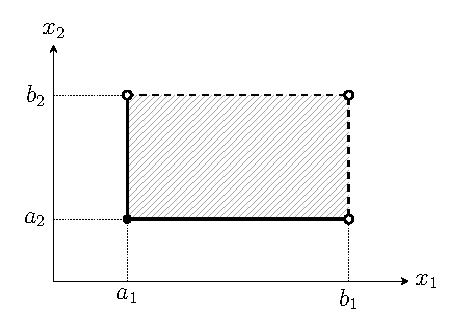
\includegraphics[width=5.4cm]{prostokat-borelowski.pdf}
  \caption{Prostokąt $[a_1,b_1)\times[a_2,b_2)$.
    Dolne końce obu przedziałów są włączone, górne wyłączone.}
  \label{fig:prostokat-borelowski}
\end{figure}

\emph{Krok 1.} Ustalmy $D\in\mathcal A^m$ i zdefiniujmy
\[
  \mathcal L_1=
  \{C\in\B(\R^n):\text{równość~\eqref{eq:niezaleznosc-blokow}
    zachodzi dla }C,D\}.
\]
Rodzina $\mathcal L_1$ jest $\lambda$-układem: zawiera $\R^n$,
jest zamknięta na różnice zbiorów zagnieżdżonych oraz na sumy
ciągów rosnących. Wynika to odpowiednio z normalizacji,
addytywności i ciągłości prawdopodobieństwa.

Jeżeli również $C\in\mathcal A^n$, to możemy zapisać
\[
  C=\prod_{i=1}^n[a_i,b_i),
  \qquad
  D=\prod_{i=n+1}^{n+m}[a_i,b_i).
\]
Z niezależności wszystkich zmiennych otrzymujemy
\begin{align*}
  \PP(X\in C,\,Y\in D)
    &=\PP\!\left(\bigcap_{i=1}^{n+m}\{X_i\in[a_i,b_i)\}\right)\\
    &=\prod_{i=1}^{n+m}\PP(X_i\in[a_i,b_i))\\
    &=\left(\prod_{i=1}^{n}\PP(X_i\in[a_i,b_i))\right)
      \left(\prod_{i=n+1}^{n+m}\PP(X_i\in[a_i,b_i))\right)\\
    &=\PP(X\in C)\PP(Y\in D).
\end{align*}
Zatem $\mathcal A^n\subseteq\mathcal L_1$. Na mocy twierdzenia
o układach $\pi$ i $\lambda$ (twierdzenie~\ref{tw:pi-lambda})
\[
  \B(\R^n)=\sigma(\mathcal A^n)\subseteq\mathcal L_1.
\]
Równość~\eqref{eq:niezaleznosc-blokow} zachodzi więc dla każdego
$C\in\B(\R^n)$ i ustalonego $D\in\mathcal A^m$.

\emph{Krok 2.} Ustalmy teraz dowolny $C\in\B(\R^n)$ i połóżmy
\[
  \mathcal L_2=
  \{D\in\B(\R^m):\text{równość~\eqref{eq:niezaleznosc-blokow}
    zachodzi dla }C,D\}.
\]
Rodzina $\mathcal L_2$ również jest $\lambda$-układem.
Z poprzedniego kroku wynika $\mathcal A^m\subseteq\mathcal L_2$.
Ponownie stosując twierdzenie~\ref{tw:pi-lambda}, dostajemy
\[
  \B(\R^m)=\sigma(\mathcal A^m)\subseteq\mathcal L_2.
\]
Dowodzi to niezależności wektorów $X$ i $Y$.

\emph{Krok 3.} Niech $f\colon\R^n\to\R$ i $g\colon\R^m\to\R$
będą borelowskie. Dla dowolnych $E,F\in\B(\R)$ przeciwobrazy
$f^{-1}(E)\in\B(\R^n)$ i $g^{-1}(F)\in\B(\R^m)$ są borelowskie.
Wobec tego
\begin{align*}
  \PP(f(X)\in E,\,g(Y)\in F)
    &=\PP\bigl(X\in f^{-1}(E),\,Y\in g^{-1}(F)\bigr)\\
    &=\PP\bigl(X\in f^{-1}(E)\bigr)
      \PP\bigl(Y\in g^{-1}(F)\bigr)\\
    &=\PP(f(X)\in E)\PP(g(Y)\in F).
\end{align*}
Zatem $f(X)$ i $g(Y)$ są niezależne.
\end{proof}
